\subsection{Использование компонентов и пресетов}
\label{sec:manual:inspector_manual}

Как говорилось ранее, основным инструментом приложения и единственным инструментом для отображения визуальной части создаваемых макетов является грид.

Применение компонентов осуществляется по алгоритму <<Drag-n-drop>>, что в переводе с английского означает буквально <<Тащи и бросай>>. Наглядно этот процесс показан на рисунке~\ref{}.

\begin{figure}[ht]
\centering
    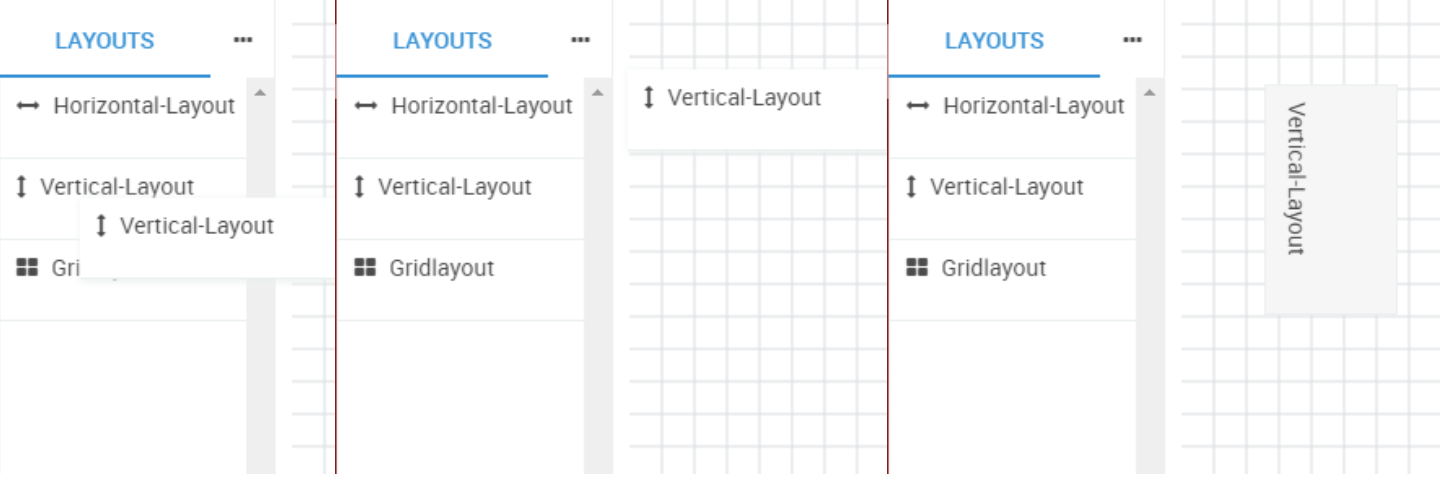
\includegraphics[scale=0.5]{manual_using_pallet.png}
    \caption{Внешний вид инспектора свойств}
    \label{sec:manual:manual_using_pallet}
\end{figure}
